% Seminar 0: Introduction
% Statistics of Financial Markets -- Bachelor's programme, Bucharest University of Economic Studies
% GENERATED by latex/build_seminar0.py -- edit the generator, not this file.
% Student version by default; the instructor version is the *_solutions.tex wrapper.
\makeatletter\@ifundefined{ifsolutions}{\expandafter\newif\csname ifsolutions\endcsname}{}\makeatother

\newcommand{\coursename}{Statistics of Financial Markets}
% Preambul comun SFM -- Statistica piețelor financiare / Statistics of Financial Markets (Beamer, 16:9)
% Același design ca MFM. Înainte de % Preambul comun SFM -- Statistica piețelor financiare / Statistics of Financial Markets (Beamer, 16:9)
% Același design ca MFM. Înainte de % Preambul comun SFM -- Statistica piețelor financiare / Statistics of Financial Markets (Beamer, 16:9)
% Același design ca MFM. Înainte de \input{../../latex/preamble} se definește
%   \newcommand{\coursename}{Statistics of Financial Markets}      (EN)
%   \newcommand{\coursename}{Statistica piețelor financiare}       (RO)  și  \def\sfmlang{ro}
% Fișierele .tex se află în EN/Courses, EN/Seminars, RO/Cursuri, RO/Seminarii (două niveluri sub rădăcină).
% Deck-urile sînt generate de latex/build_chapterN.py / build_seminarN.py (vezi latex/sfm_build.py).

\documentclass[9pt, aspectratio=169, t]{beamer}
\providecommand{\coursename}{Statistics of Financial Markets}

% Ensure content fits on slides
\setbeamersize{text margin left=8mm, text margin right=8mm}

%=============================================================================
% THEME AND STYLE CONFIGURATION
%=============================================================================
\usetheme{default}
% Using default theme for clean header/footer control

% Color Palette (matching Redispatch PDF)
\definecolor{MainBlue}{RGB}{26, 58, 110}
\definecolor{AccentBlue}{RGB}{26, 58, 110}
\definecolor{IDAred}{RGB}{205, 0, 0}
\definecolor{DarkGray}{RGB}{51, 51, 51}
\definecolor{MediumGray}{RGB}{128, 128, 128}
\definecolor{LightGray}{RGB}{248, 248, 248}
\definecolor{VeryLightGray}{RGB}{235, 235, 235}
\definecolor{KeynoteGray}{RGB}{218, 218, 218}
\definecolor{SectionGray}{RGB}{120, 120, 120}
\definecolor{FooterGray}{RGB}{100, 100, 100}
\definecolor{Crimson}{RGB}{220, 53, 69}
\definecolor{Forest}{RGB}{46, 125, 50}
\definecolor{Amber}{RGB}{181, 133, 63}
\definecolor{Orange}{RGB}{230, 126, 34}
\definecolor{Purple}{RGB}{142, 68, 173}

% Gradient background (exact Keynote 315° gradient: white to RGB 218,218,218)
\setbeamertemplate{background}{%
    \begin{tikzpicture}[remember picture, overlay]
        \shade[shading=axis, shading angle=315,
        top color=white, bottom color=KeynoteGray]
        (current page.south west) rectangle (current page.north east);
    \end{tikzpicture}%
}
% Fallback solid color for compatibility
\setbeamercolor{background canvas}{bg=}

\setbeamercolor{palette primary}{bg=MainBlue, fg=white}
\setbeamercolor{palette secondary}{bg=MainBlue!85, fg=white}
\setbeamercolor{palette tertiary}{bg=MainBlue!70, fg=white}
\setbeamercolor{structure}{fg=MainBlue}
\setbeamercolor{title}{fg=IDAred}
\setbeamercolor{frametitle}{fg=IDAred, bg=}
\setbeamercolor{block title}{bg=MainBlue, fg=white}
\setbeamercolor{block body}{bg=VeryLightGray, fg=DarkGray}
\setbeamercolor{block title alerted}{bg=Crimson, fg=white}
\setbeamercolor{block body alerted}{bg=Crimson!8, fg=DarkGray}
\setbeamercolor{block title example}{bg=Forest, fg=white}
\setbeamercolor{block body example}{bg=Forest!8, fg=DarkGray}
\setbeamercolor{item}{fg=MainBlue}

% Footer colors (override Madrid theme blue)
\setbeamercolor{author in head/foot}{fg=FooterGray, bg=}
\setbeamercolor{title in head/foot}{fg=FooterGray, bg=}
\setbeamercolor{date in head/foot}{fg=FooterGray, bg=}
\setbeamercolor{section in head/foot}{fg=FooterGray, bg=}
\setbeamercolor{subsection in head/foot}{fg=FooterGray, bg=}

% Bullet styles (apply everywhere including blocks)
\setbeamertemplate{itemize item}{\color{MainBlue}$\boxdot$}
\setbeamertemplate{itemize subitem}{\color{MainBlue}$\blacktriangleright$}
\setbeamertemplate{itemize subsubitem}{\color{MainBlue}\tiny$\bullet$}
\setbeamertemplate{itemize/enumerate body begin}{\normalsize}
\setbeamertemplate{itemize/enumerate subbody begin}{\normalsize}

% Item spacing - compact style
\setlength{\leftmargini}{10pt}       % Level 1: minimal indent
\setlength{\leftmarginii}{10pt}      % Level 2: minimal additional indent
% Compact list spacing (zero extra space before/after lists in blocks)
\makeatletter
\def\@listi{\leftmargin\leftmargini \topsep 0pt \parsep 0pt \itemsep 0pt}
\def\@listii{\leftmargin\leftmarginii \topsep 0pt \parsep 0pt \itemsep 0pt}
\makeatother

\setbeamertemplate{navigation symbols}{}

%=============================================================================
% CUSTOM HEADLINE
%=============================================================================
\setbeamertemplate{headline}{%
    \vskip10pt%
    \hbox to \paperwidth{%
        \hskip0.5cm%
        {\small\color{FooterGray}\renewcommand{\hyperlink}[2]{##2}\insertsectionhead}%
        \hfill%
        \textcolor{FooterGray}{\small\insertframenumber}%
        \hskip0.5cm%
    }%
    \vskip4pt%
    {\color{FooterGray}\hrule height 0.4pt}%
}

%=============================================================================
% CUSTOM FOOTER
%=============================================================================
\usepackage{fontawesome5}

\setbeamertemplate{footline}{%
    {\color{FooterGray}\hrule height 0.4pt}%
    \vskip4pt%
    \hbox to \paperwidth{%
        \hskip0.5cm%
        \textcolor{FooterGray}{\small\coursename}%
        \hfill%
        \raisebox{-0.1em}{%
            \begin{tikzpicture}[x=0.08em, y=0.08em, line width=0.4pt]
                \draw[FooterGray] (0,3) -- (1,4) -- (2,3.5) -- (3,5) -- (4,4) -- (5,6) -- (6,5.5) -- (7,4) -- (8,5) -- (9,7) -- (10,6) -- (11,5) -- (12,6.5) -- (13,8) -- (14,7) -- (15,6) -- (16,7.5) -- (17,9) -- (18,8) -- (19,7) -- (20,8.5) -- (21,10) -- (22,9) -- (23,8) -- (24,9.5);
            \end{tikzpicture}%
        }%
        \hskip0.5cm%
    }%
    \vskip6pt%
}

%=============================================================================
% PACKAGES
%=============================================================================
\usepackage[utf8]{inputenc}
\DeclareUnicodeCharacter{03B1}{\ensuremath{\alpha}}
\usepackage[T1]{fontenc}
\usepackage{amsmath, amssymb, amsthm}
\usepackage{mathtools}
\usepackage{bm}
\usepackage{tikz}
\usetikzlibrary{arrows.meta, positioning, shapes, calc, decorations.pathreplacing, shadings}
\usepackage{booktabs}
\usepackage{multirow}
\usepackage{array}
\usepackage{graphicx}
\usepackage{hyperref}
\usepackage{colortbl}
\usepackage{listings}
\lstset{language=Python, basicstyle=\ttfamily\scriptsize, keywordstyle=\color{MainBlue}\bfseries,
  commentstyle=\color{Forest}, stringstyle=\color{Crimson}, breaklines=true,
  frame=none, backgroundcolor=\color{VeryLightGray}, xleftmargin=2mm}
\hypersetup{colorlinks=true, linkcolor=MainBlue, urlcolor=MainBlue}
\graphicspath{{../../logos/}{../../charts/}{../../photos/}}
\usepackage{xcolor}
\hfuzz=2pt  % Suppress tiny overfull warnings (<2pt)
\vfuzz=2pt  % Suppress tiny vertical overfull warnings (<2pt)

%=============================================================================
% QUANTLET COMMANDS
%   \quantlet{<displayed name>}{<url>}       (generic, compatible with the older SFM decks)
%   \sfmquantlet{Ch_05}{SFM_ch5_garch}       -> https://github.com/danpele/SFM/tree/main/Quantlets/Ch_05/SFM_ch5_garch
%   \qlurl{<folder>} is defined per chapter by the generator (Quantlets/Ch_NN/<folder>)
%=============================================================================
\newcommand{\sfmrepo}{https://github.com/danpele/SFM}
\newcommand{\sfmqlbase}{https://github.com/danpele/SFM/tree/main/Quantlets}
\newcommand{\quantlet}[2]{%
    \hfill\href{#2}{%
        \raisebox{-0.15em}{
\includegraphics[height=0.7em]{ql_logo.png}}%
        \textcolor{MainBlue}{\tiny\ #1}%
    }%
}
\newcommand{\sfmquantlet}[2]{\quantlet{\detokenize{#2}}{\sfmqlbase/#1/#2}}

%=============================================================================
% NOTEBOOKS (Google Colab)
%   \colaburl{notebooks/EN/chapter5_seminar_notebook.ipynb} -> the Colab link of a file in the SFM repo
%   \nb: the chapter notebook (each seminar deck redefines it with \renewcommand)
%=============================================================================
\newcommand{\colaburl}[1]{https://colab.research.google.com/github/danpele/SFM/blob/main/#1}
\newcommand{\nb}{https://colab.research.google.com/github/danpele/SFM/tree/main/notebooks/EN}
\newcommand{\nbname}{notebooks/EN}

%=============================================================================
% SLIDE HELPERS (used by the generators; the same as in MFM)
%=============================================================================
% local font size for list bodies (the preamble forces \normalsize)
\newcommand{\itemsize}[1]{\setbeamertemplate{itemize/enumerate body begin}{#1}\setbeamertemplate{itemize/enumerate subbody begin}{#1}}
\newcommand{\intitle}[1]{{\hypersetup{urlcolor=white}#1}}   % white links inside coloured title bars
\newcommand{\imgcap}[1]{{\scriptsize #1}\\[0.5mm]}          % caption under a photo
\newcommand{\imgcredit}[2]{{\tiny\color{FooterGray}\href{#1}{#2}}}   % image credit: source URL, author/licence
\newcommand{\aiprompt}[1]{{\ttfamily\color{MainBlue}#1}}     % a prompt to an AI assistant

%=============================================================================
% SEMINARS: student version by default; the instructor wrapper *_solutions.tex sets \solutionstrue
%=============================================================================
\makeatletter\@ifundefined{ifsolutions}{\expandafter\newif\csname ifsolutions\endcsname}{}\makeatother
\newcommand{\solonly}[1]{\ifsolutions #1\fi}
\newcommand{\propsub}{\ifsolutions\else\framesubtitle{\ifdefined\sfmlang Rezolvarea se discută la seminar\else Solution discussed in class\fi}\fi}

%=============================================================================
% APPENDIX AND CHAPTER LINKS (latex/appendix_links.py writes the calls; it also re-declares these
% macros before \begin{document}, so the decks compile with or without this preamble block)
%=============================================================================
\providecommand{\sfmapplink}[3]{\hypertarget{#2}{}\hyperlink{#1}{\beamergotobutton{#3}}}
\providecommand{\sfmappback}[2]{\begin{tikzpicture}[remember picture,overlay]\node[anchor=south east] at ([xshift=-3mm,yshift=7mm]current page.south east){\hyperlink{#1}{\beamerreturnbutton{#2}}};\end{tikzpicture}}
\providecommand{\sfmchlink}[2]{\href{#1}{#2}}
\providecommand{\sfmchlinkt}[2]{\href{#1}{\usebeamercolor[fg]{frametitle}#2}}

%=============================================================================
% QUANTINAR COMMAND: link către un curs Quantinar (subiecte avansate)
%=============================================================================
\newcommand{\quantinar}[2]{%
    \href{#2}{%
        \raisebox{-0.15em}{
\includegraphics[height=0.8em]{qr_logo.png}}%
        \textcolor{MainBlue}{\scriptsize\ #1}%
    }%
}

%=============================================================================
% CUSTOM TITLE PAGE
%=============================================================================
\defbeamertemplate*{title page}{hybrid}[1][]
{
    \vspace{0.2cm}
    % Logos row - top header (with clickable links)
    \begin{center}
        \href{https://www.ase.ro}{
\includegraphics[height=1.0cm]{ase_logo.png}}\hspace{0.3cm}%
        \href{https://theida.net}{
\includegraphics[height=1.0cm]{ida_logo.png}}\hspace{0.3cm}%
        \href{https://blockchain-research-center.com}{
\includegraphics[height=1.0cm]{brc_logo.png}}\hspace{0.3cm}%
        \href{https://www.ai4efin.ase.ro}{
\includegraphics[height=1.0cm]{ai4efin_logo.png}}\hspace{0.3cm}%
        \href{https://ipe.ro/new}{
\includegraphics[height=1.0cm]{acad_logo.png}}\hspace{0.3cm}%
        \href{https://www.digital-finance-msca.com}{
\includegraphics[height=1.0cm]{msca_logo.png}}%
    \end{center}

    \vspace{0.6cm}

    % Main title with Q logos on sides (with clickable links)
    \begin{center}
        \begin{minipage}{0.1\textwidth}
            \centering
            \href{https://quantlet.com}{
\includegraphics[height=1.1cm]{ql_logo.png}}
        \end{minipage}%
        \begin{minipage}{0.78\textwidth}
            \centering
            {\LARGE\bfseries\usebeamercolor[fg]{title}\inserttitle}

            \vspace{0.3cm}

            {\usebeamerfont{subtitle}\usebeamercolor[fg]{title}\insertsubtitle}
        \end{minipage}%
        \begin{minipage}{0.1\textwidth}
            \centering
            \href{https://quantinar.com}{
\includegraphics[height=1.1cm]{qr_logo.png}}
        \end{minipage}
    \end{center}

    \vspace{0.6cm}

    % Authors (left aligned)
    \hspace{0.5cm}{\usebeamerfont{author}\insertauthor}

    \vspace{0.3cm}

    % Institute/Affiliations (left aligned)
    \hspace{0.5cm}\begin{minipage}[t]{0.9\textwidth}
        \raggedright\small\insertinstitute
    \end{minipage}
}

%=============================================================================
% THEOREM ENVIRONMENTS
%=============================================================================
\theoremstyle{definition}
\setbeamertemplate{theorems}[numbered]
\ifdefined\sfmlang
\newtheorem{defn}{Definiție}
\newtheorem{thm}{Teoremă}
\newtheorem{prop}{Propoziție}
\newtheorem{rmk}{Observație}
\else
\newtheorem{defn}{Definition}
\newtheorem{thm}{Theorem}
\newtheorem{prop}{Proposition}
\newtheorem{rmk}{Remark}
\fi

%=============================================================================
% CENTRED MINIPAGE (no extra vertical space)
%=============================================================================
\newenvironment{cminipage}[1]{%
    \par\noindent\hfill\begin{minipage}{#1}\ignorespaces
}{%
    \end{minipage}\hfill\null\par
}

%=============================================================================
% CUSTOM COMMANDS
%=============================================================================
\newcommand{\E}{\mathbb{E}}
\newcommand{\Var}{\text{Var}}
\newcommand{\Cov}{\text{Cov}}
\newcommand{\Corr}{\text{Corr}}
\newcommand{\R}{\mathbb{R}}
\newcommand{\N}{\mathbb{N}}
\newcommand{\Z}{\mathbb{Z}}
\newcommand{\B}{\mathbf{B}}
\newcommand{\imark}{\textcolor{MainBlue}{\textbullet}}
\newcommand{\RMSE}{\text{RMSE}}
\newcommand{\MAE}{\text{MAE}}
\newcommand{\MAPE}{\text{MAPE}}

 se definește
%   \newcommand{\coursename}{Statistics of Financial Markets}      (EN)
%   \newcommand{\coursename}{Statistica piețelor financiare}       (RO)  și  \def\sfmlang{ro}
% Fișierele .tex se află în EN/Courses, EN/Seminars, RO/Cursuri, RO/Seminarii (două niveluri sub rădăcină).
% Deck-urile sînt generate de latex/build_chapterN.py / build_seminarN.py (vezi latex/sfm_build.py).

\documentclass[9pt, aspectratio=169, t]{beamer}
\providecommand{\coursename}{Statistics of Financial Markets}

% Ensure content fits on slides
\setbeamersize{text margin left=8mm, text margin right=8mm}

%=============================================================================
% THEME AND STYLE CONFIGURATION
%=============================================================================
\usetheme{default}
% Using default theme for clean header/footer control

% Color Palette (matching Redispatch PDF)
\definecolor{MainBlue}{RGB}{26, 58, 110}
\definecolor{AccentBlue}{RGB}{26, 58, 110}
\definecolor{IDAred}{RGB}{205, 0, 0}
\definecolor{DarkGray}{RGB}{51, 51, 51}
\definecolor{MediumGray}{RGB}{128, 128, 128}
\definecolor{LightGray}{RGB}{248, 248, 248}
\definecolor{VeryLightGray}{RGB}{235, 235, 235}
\definecolor{KeynoteGray}{RGB}{218, 218, 218}
\definecolor{SectionGray}{RGB}{120, 120, 120}
\definecolor{FooterGray}{RGB}{100, 100, 100}
\definecolor{Crimson}{RGB}{220, 53, 69}
\definecolor{Forest}{RGB}{46, 125, 50}
\definecolor{Amber}{RGB}{181, 133, 63}
\definecolor{Orange}{RGB}{230, 126, 34}
\definecolor{Purple}{RGB}{142, 68, 173}

% Gradient background (exact Keynote 315° gradient: white to RGB 218,218,218)
\setbeamertemplate{background}{%
    \begin{tikzpicture}[remember picture, overlay]
        \shade[shading=axis, shading angle=315,
        top color=white, bottom color=KeynoteGray]
        (current page.south west) rectangle (current page.north east);
    \end{tikzpicture}%
}
% Fallback solid color for compatibility
\setbeamercolor{background canvas}{bg=}

\setbeamercolor{palette primary}{bg=MainBlue, fg=white}
\setbeamercolor{palette secondary}{bg=MainBlue!85, fg=white}
\setbeamercolor{palette tertiary}{bg=MainBlue!70, fg=white}
\setbeamercolor{structure}{fg=MainBlue}
\setbeamercolor{title}{fg=IDAred}
\setbeamercolor{frametitle}{fg=IDAred, bg=}
\setbeamercolor{block title}{bg=MainBlue, fg=white}
\setbeamercolor{block body}{bg=VeryLightGray, fg=DarkGray}
\setbeamercolor{block title alerted}{bg=Crimson, fg=white}
\setbeamercolor{block body alerted}{bg=Crimson!8, fg=DarkGray}
\setbeamercolor{block title example}{bg=Forest, fg=white}
\setbeamercolor{block body example}{bg=Forest!8, fg=DarkGray}
\setbeamercolor{item}{fg=MainBlue}

% Footer colors (override Madrid theme blue)
\setbeamercolor{author in head/foot}{fg=FooterGray, bg=}
\setbeamercolor{title in head/foot}{fg=FooterGray, bg=}
\setbeamercolor{date in head/foot}{fg=FooterGray, bg=}
\setbeamercolor{section in head/foot}{fg=FooterGray, bg=}
\setbeamercolor{subsection in head/foot}{fg=FooterGray, bg=}

% Bullet styles (apply everywhere including blocks)
\setbeamertemplate{itemize item}{\color{MainBlue}$\boxdot$}
\setbeamertemplate{itemize subitem}{\color{MainBlue}$\blacktriangleright$}
\setbeamertemplate{itemize subsubitem}{\color{MainBlue}\tiny$\bullet$}
\setbeamertemplate{itemize/enumerate body begin}{\normalsize}
\setbeamertemplate{itemize/enumerate subbody begin}{\normalsize}

% Item spacing - compact style
\setlength{\leftmargini}{10pt}       % Level 1: minimal indent
\setlength{\leftmarginii}{10pt}      % Level 2: minimal additional indent
% Compact list spacing (zero extra space before/after lists in blocks)
\makeatletter
\def\@listi{\leftmargin\leftmargini \topsep 0pt \parsep 0pt \itemsep 0pt}
\def\@listii{\leftmargin\leftmarginii \topsep 0pt \parsep 0pt \itemsep 0pt}
\makeatother

\setbeamertemplate{navigation symbols}{}

%=============================================================================
% CUSTOM HEADLINE
%=============================================================================
\setbeamertemplate{headline}{%
    \vskip10pt%
    \hbox to \paperwidth{%
        \hskip0.5cm%
        {\small\color{FooterGray}\renewcommand{\hyperlink}[2]{##2}\insertsectionhead}%
        \hfill%
        \textcolor{FooterGray}{\small\insertframenumber}%
        \hskip0.5cm%
    }%
    \vskip4pt%
    {\color{FooterGray}\hrule height 0.4pt}%
}

%=============================================================================
% CUSTOM FOOTER
%=============================================================================
\usepackage{fontawesome5}

\setbeamertemplate{footline}{%
    {\color{FooterGray}\hrule height 0.4pt}%
    \vskip4pt%
    \hbox to \paperwidth{%
        \hskip0.5cm%
        \textcolor{FooterGray}{\small\coursename}%
        \hfill%
        \raisebox{-0.1em}{%
            \begin{tikzpicture}[x=0.08em, y=0.08em, line width=0.4pt]
                \draw[FooterGray] (0,3) -- (1,4) -- (2,3.5) -- (3,5) -- (4,4) -- (5,6) -- (6,5.5) -- (7,4) -- (8,5) -- (9,7) -- (10,6) -- (11,5) -- (12,6.5) -- (13,8) -- (14,7) -- (15,6) -- (16,7.5) -- (17,9) -- (18,8) -- (19,7) -- (20,8.5) -- (21,10) -- (22,9) -- (23,8) -- (24,9.5);
            \end{tikzpicture}%
        }%
        \hskip0.5cm%
    }%
    \vskip6pt%
}

%=============================================================================
% PACKAGES
%=============================================================================
\usepackage[utf8]{inputenc}
\DeclareUnicodeCharacter{03B1}{\ensuremath{\alpha}}
\usepackage[T1]{fontenc}
\usepackage{amsmath, amssymb, amsthm}
\usepackage{mathtools}
\usepackage{bm}
\usepackage{tikz}
\usetikzlibrary{arrows.meta, positioning, shapes, calc, decorations.pathreplacing, shadings}
\usepackage{booktabs}
\usepackage{multirow}
\usepackage{array}
\usepackage{graphicx}
\usepackage{hyperref}
\usepackage{colortbl}
\usepackage{listings}
\lstset{language=Python, basicstyle=\ttfamily\scriptsize, keywordstyle=\color{MainBlue}\bfseries,
  commentstyle=\color{Forest}, stringstyle=\color{Crimson}, breaklines=true,
  frame=none, backgroundcolor=\color{VeryLightGray}, xleftmargin=2mm}
\hypersetup{colorlinks=true, linkcolor=MainBlue, urlcolor=MainBlue}
\graphicspath{{../../logos/}{../../charts/}{../../photos/}}
\usepackage{xcolor}
\hfuzz=2pt  % Suppress tiny overfull warnings (<2pt)
\vfuzz=2pt  % Suppress tiny vertical overfull warnings (<2pt)

%=============================================================================
% QUANTLET COMMANDS
%   \quantlet{<displayed name>}{<url>}       (generic, compatible with the older SFM decks)
%   \sfmquantlet{Ch_05}{SFM_ch5_garch}       -> https://github.com/danpele/SFM/tree/main/Quantlets/Ch_05/SFM_ch5_garch
%   \qlurl{<folder>} is defined per chapter by the generator (Quantlets/Ch_NN/<folder>)
%=============================================================================
\newcommand{\sfmrepo}{https://github.com/danpele/SFM}
\newcommand{\sfmqlbase}{https://github.com/danpele/SFM/tree/main/Quantlets}
\newcommand{\quantlet}[2]{%
    \hfill\href{#2}{%
        \raisebox{-0.15em}{
\includegraphics[height=0.7em]{ql_logo.png}}%
        \textcolor{MainBlue}{\tiny\ #1}%
    }%
}
\newcommand{\sfmquantlet}[2]{\quantlet{\detokenize{#2}}{\sfmqlbase/#1/#2}}

%=============================================================================
% NOTEBOOKS (Google Colab)
%   \colaburl{notebooks/EN/chapter5_seminar_notebook.ipynb} -> the Colab link of a file in the SFM repo
%   \nb: the chapter notebook (each seminar deck redefines it with \renewcommand)
%=============================================================================
\newcommand{\colaburl}[1]{https://colab.research.google.com/github/danpele/SFM/blob/main/#1}
\newcommand{\nb}{https://colab.research.google.com/github/danpele/SFM/tree/main/notebooks/EN}
\newcommand{\nbname}{notebooks/EN}

%=============================================================================
% SLIDE HELPERS (used by the generators; the same as in MFM)
%=============================================================================
% local font size for list bodies (the preamble forces \normalsize)
\newcommand{\itemsize}[1]{\setbeamertemplate{itemize/enumerate body begin}{#1}\setbeamertemplate{itemize/enumerate subbody begin}{#1}}
\newcommand{\intitle}[1]{{\hypersetup{urlcolor=white}#1}}   % white links inside coloured title bars
\newcommand{\imgcap}[1]{{\scriptsize #1}\\[0.5mm]}          % caption under a photo
\newcommand{\imgcredit}[2]{{\tiny\color{FooterGray}\href{#1}{#2}}}   % image credit: source URL, author/licence
\newcommand{\aiprompt}[1]{{\ttfamily\color{MainBlue}#1}}     % a prompt to an AI assistant

%=============================================================================
% SEMINARS: student version by default; the instructor wrapper *_solutions.tex sets \solutionstrue
%=============================================================================
\makeatletter\@ifundefined{ifsolutions}{\expandafter\newif\csname ifsolutions\endcsname}{}\makeatother
\newcommand{\solonly}[1]{\ifsolutions #1\fi}
\newcommand{\propsub}{\ifsolutions\else\framesubtitle{\ifdefined\sfmlang Rezolvarea se discută la seminar\else Solution discussed in class\fi}\fi}

%=============================================================================
% APPENDIX AND CHAPTER LINKS (latex/appendix_links.py writes the calls; it also re-declares these
% macros before \begin{document}, so the decks compile with or without this preamble block)
%=============================================================================
\providecommand{\sfmapplink}[3]{\hypertarget{#2}{}\hyperlink{#1}{\beamergotobutton{#3}}}
\providecommand{\sfmappback}[2]{\begin{tikzpicture}[remember picture,overlay]\node[anchor=south east] at ([xshift=-3mm,yshift=7mm]current page.south east){\hyperlink{#1}{\beamerreturnbutton{#2}}};\end{tikzpicture}}
\providecommand{\sfmchlink}[2]{\href{#1}{#2}}
\providecommand{\sfmchlinkt}[2]{\href{#1}{\usebeamercolor[fg]{frametitle}#2}}

%=============================================================================
% QUANTINAR COMMAND: link către un curs Quantinar (subiecte avansate)
%=============================================================================
\newcommand{\quantinar}[2]{%
    \href{#2}{%
        \raisebox{-0.15em}{
\includegraphics[height=0.8em]{qr_logo.png}}%
        \textcolor{MainBlue}{\scriptsize\ #1}%
    }%
}

%=============================================================================
% CUSTOM TITLE PAGE
%=============================================================================
\defbeamertemplate*{title page}{hybrid}[1][]
{
    \vspace{0.2cm}
    % Logos row - top header (with clickable links)
    \begin{center}
        \href{https://www.ase.ro}{
\includegraphics[height=1.0cm]{ase_logo.png}}\hspace{0.3cm}%
        \href{https://theida.net}{
\includegraphics[height=1.0cm]{ida_logo.png}}\hspace{0.3cm}%
        \href{https://blockchain-research-center.com}{
\includegraphics[height=1.0cm]{brc_logo.png}}\hspace{0.3cm}%
        \href{https://www.ai4efin.ase.ro}{
\includegraphics[height=1.0cm]{ai4efin_logo.png}}\hspace{0.3cm}%
        \href{https://ipe.ro/new}{
\includegraphics[height=1.0cm]{acad_logo.png}}\hspace{0.3cm}%
        \href{https://www.digital-finance-msca.com}{
\includegraphics[height=1.0cm]{msca_logo.png}}%
    \end{center}

    \vspace{0.6cm}

    % Main title with Q logos on sides (with clickable links)
    \begin{center}
        \begin{minipage}{0.1\textwidth}
            \centering
            \href{https://quantlet.com}{
\includegraphics[height=1.1cm]{ql_logo.png}}
        \end{minipage}%
        \begin{minipage}{0.78\textwidth}
            \centering
            {\LARGE\bfseries\usebeamercolor[fg]{title}\inserttitle}

            \vspace{0.3cm}

            {\usebeamerfont{subtitle}\usebeamercolor[fg]{title}\insertsubtitle}
        \end{minipage}%
        \begin{minipage}{0.1\textwidth}
            \centering
            \href{https://quantinar.com}{
\includegraphics[height=1.1cm]{qr_logo.png}}
        \end{minipage}
    \end{center}

    \vspace{0.6cm}

    % Authors (left aligned)
    \hspace{0.5cm}{\usebeamerfont{author}\insertauthor}

    \vspace{0.3cm}

    % Institute/Affiliations (left aligned)
    \hspace{0.5cm}\begin{minipage}[t]{0.9\textwidth}
        \raggedright\small\insertinstitute
    \end{minipage}
}

%=============================================================================
% THEOREM ENVIRONMENTS
%=============================================================================
\theoremstyle{definition}
\setbeamertemplate{theorems}[numbered]
\ifdefined\sfmlang
\newtheorem{defn}{Definiție}
\newtheorem{thm}{Teoremă}
\newtheorem{prop}{Propoziție}
\newtheorem{rmk}{Observație}
\else
\newtheorem{defn}{Definition}
\newtheorem{thm}{Theorem}
\newtheorem{prop}{Proposition}
\newtheorem{rmk}{Remark}
\fi

%=============================================================================
% CENTRED MINIPAGE (no extra vertical space)
%=============================================================================
\newenvironment{cminipage}[1]{%
    \par\noindent\hfill\begin{minipage}{#1}\ignorespaces
}{%
    \end{minipage}\hfill\null\par
}

%=============================================================================
% CUSTOM COMMANDS
%=============================================================================
\newcommand{\E}{\mathbb{E}}
\newcommand{\Var}{\text{Var}}
\newcommand{\Cov}{\text{Cov}}
\newcommand{\Corr}{\text{Corr}}
\newcommand{\R}{\mathbb{R}}
\newcommand{\N}{\mathbb{N}}
\newcommand{\Z}{\mathbb{Z}}
\newcommand{\B}{\mathbf{B}}
\newcommand{\imark}{\textcolor{MainBlue}{\textbullet}}
\newcommand{\RMSE}{\text{RMSE}}
\newcommand{\MAE}{\text{MAE}}
\newcommand{\MAPE}{\text{MAPE}}

 se definește
%   \newcommand{\coursename}{Statistics of Financial Markets}      (EN)
%   \newcommand{\coursename}{Statistica piețelor financiare}       (RO)  și  \def\sfmlang{ro}
% Fișierele .tex se află în EN/Courses, EN/Seminars, RO/Cursuri, RO/Seminarii (două niveluri sub rădăcină).
% Deck-urile sînt generate de latex/build_chapterN.py / build_seminarN.py (vezi latex/sfm_build.py).

\documentclass[9pt, aspectratio=169, t]{beamer}
\providecommand{\coursename}{Statistics of Financial Markets}

% Ensure content fits on slides
\setbeamersize{text margin left=8mm, text margin right=8mm}

%=============================================================================
% THEME AND STYLE CONFIGURATION
%=============================================================================
\usetheme{default}
% Using default theme for clean header/footer control

% Color Palette (matching Redispatch PDF)
\definecolor{MainBlue}{RGB}{26, 58, 110}
\definecolor{AccentBlue}{RGB}{26, 58, 110}
\definecolor{IDAred}{RGB}{205, 0, 0}
\definecolor{DarkGray}{RGB}{51, 51, 51}
\definecolor{MediumGray}{RGB}{128, 128, 128}
\definecolor{LightGray}{RGB}{248, 248, 248}
\definecolor{VeryLightGray}{RGB}{235, 235, 235}
\definecolor{KeynoteGray}{RGB}{218, 218, 218}
\definecolor{SectionGray}{RGB}{120, 120, 120}
\definecolor{FooterGray}{RGB}{100, 100, 100}
\definecolor{Crimson}{RGB}{220, 53, 69}
\definecolor{Forest}{RGB}{46, 125, 50}
\definecolor{Amber}{RGB}{181, 133, 63}
\definecolor{Orange}{RGB}{230, 126, 34}
\definecolor{Purple}{RGB}{142, 68, 173}

% Gradient background (exact Keynote 315° gradient: white to RGB 218,218,218)
\setbeamertemplate{background}{%
    \begin{tikzpicture}[remember picture, overlay]
        \shade[shading=axis, shading angle=315,
        top color=white, bottom color=KeynoteGray]
        (current page.south west) rectangle (current page.north east);
    \end{tikzpicture}%
}
% Fallback solid color for compatibility
\setbeamercolor{background canvas}{bg=}

\setbeamercolor{palette primary}{bg=MainBlue, fg=white}
\setbeamercolor{palette secondary}{bg=MainBlue!85, fg=white}
\setbeamercolor{palette tertiary}{bg=MainBlue!70, fg=white}
\setbeamercolor{structure}{fg=MainBlue}
\setbeamercolor{title}{fg=IDAred}
\setbeamercolor{frametitle}{fg=IDAred, bg=}
\setbeamercolor{block title}{bg=MainBlue, fg=white}
\setbeamercolor{block body}{bg=VeryLightGray, fg=DarkGray}
\setbeamercolor{block title alerted}{bg=Crimson, fg=white}
\setbeamercolor{block body alerted}{bg=Crimson!8, fg=DarkGray}
\setbeamercolor{block title example}{bg=Forest, fg=white}
\setbeamercolor{block body example}{bg=Forest!8, fg=DarkGray}
\setbeamercolor{item}{fg=MainBlue}

% Footer colors (override Madrid theme blue)
\setbeamercolor{author in head/foot}{fg=FooterGray, bg=}
\setbeamercolor{title in head/foot}{fg=FooterGray, bg=}
\setbeamercolor{date in head/foot}{fg=FooterGray, bg=}
\setbeamercolor{section in head/foot}{fg=FooterGray, bg=}
\setbeamercolor{subsection in head/foot}{fg=FooterGray, bg=}

% Bullet styles (apply everywhere including blocks)
\setbeamertemplate{itemize item}{\color{MainBlue}$\boxdot$}
\setbeamertemplate{itemize subitem}{\color{MainBlue}$\blacktriangleright$}
\setbeamertemplate{itemize subsubitem}{\color{MainBlue}\tiny$\bullet$}
\setbeamertemplate{itemize/enumerate body begin}{\normalsize}
\setbeamertemplate{itemize/enumerate subbody begin}{\normalsize}

% Item spacing - compact style
\setlength{\leftmargini}{10pt}       % Level 1: minimal indent
\setlength{\leftmarginii}{10pt}      % Level 2: minimal additional indent
% Compact list spacing (zero extra space before/after lists in blocks)
\makeatletter
\def\@listi{\leftmargin\leftmargini \topsep 0pt \parsep 0pt \itemsep 0pt}
\def\@listii{\leftmargin\leftmarginii \topsep 0pt \parsep 0pt \itemsep 0pt}
\makeatother

\setbeamertemplate{navigation symbols}{}

%=============================================================================
% CUSTOM HEADLINE
%=============================================================================
\setbeamertemplate{headline}{%
    \vskip10pt%
    \hbox to \paperwidth{%
        \hskip0.5cm%
        {\small\color{FooterGray}\renewcommand{\hyperlink}[2]{##2}\insertsectionhead}%
        \hfill%
        \textcolor{FooterGray}{\small\insertframenumber}%
        \hskip0.5cm%
    }%
    \vskip4pt%
    {\color{FooterGray}\hrule height 0.4pt}%
}

%=============================================================================
% CUSTOM FOOTER
%=============================================================================
\usepackage{fontawesome5}

\setbeamertemplate{footline}{%
    {\color{FooterGray}\hrule height 0.4pt}%
    \vskip4pt%
    \hbox to \paperwidth{%
        \hskip0.5cm%
        \textcolor{FooterGray}{\small\coursename}%
        \hfill%
        \raisebox{-0.1em}{%
            \begin{tikzpicture}[x=0.08em, y=0.08em, line width=0.4pt]
                \draw[FooterGray] (0,3) -- (1,4) -- (2,3.5) -- (3,5) -- (4,4) -- (5,6) -- (6,5.5) -- (7,4) -- (8,5) -- (9,7) -- (10,6) -- (11,5) -- (12,6.5) -- (13,8) -- (14,7) -- (15,6) -- (16,7.5) -- (17,9) -- (18,8) -- (19,7) -- (20,8.5) -- (21,10) -- (22,9) -- (23,8) -- (24,9.5);
            \end{tikzpicture}%
        }%
        \hskip0.5cm%
    }%
    \vskip6pt%
}

%=============================================================================
% PACKAGES
%=============================================================================
\usepackage[utf8]{inputenc}
\DeclareUnicodeCharacter{03B1}{\ensuremath{\alpha}}
\usepackage[T1]{fontenc}
\usepackage{amsmath, amssymb, amsthm}
\usepackage{mathtools}
\usepackage{bm}
\usepackage{tikz}
\usetikzlibrary{arrows.meta, positioning, shapes, calc, decorations.pathreplacing, shadings}
\usepackage{booktabs}
\usepackage{multirow}
\usepackage{array}
\usepackage{graphicx}
\usepackage{hyperref}
\usepackage{colortbl}
\usepackage{listings}
\lstset{language=Python, basicstyle=\ttfamily\scriptsize, keywordstyle=\color{MainBlue}\bfseries,
  commentstyle=\color{Forest}, stringstyle=\color{Crimson}, breaklines=true,
  frame=none, backgroundcolor=\color{VeryLightGray}, xleftmargin=2mm}
\hypersetup{colorlinks=true, linkcolor=MainBlue, urlcolor=MainBlue}
\graphicspath{{../../logos/}{../../charts/}{../../photos/}}
\usepackage{xcolor}
\hfuzz=2pt  % Suppress tiny overfull warnings (<2pt)
\vfuzz=2pt  % Suppress tiny vertical overfull warnings (<2pt)

%=============================================================================
% QUANTLET COMMANDS
%   \quantlet{<displayed name>}{<url>}       (generic, compatible with the older SFM decks)
%   \sfmquantlet{Ch_05}{SFM_ch5_garch}       -> https://github.com/danpele/SFM/tree/main/Quantlets/Ch_05/SFM_ch5_garch
%   \qlurl{<folder>} is defined per chapter by the generator (Quantlets/Ch_NN/<folder>)
%=============================================================================
\newcommand{\sfmrepo}{https://github.com/danpele/SFM}
\newcommand{\sfmqlbase}{https://github.com/danpele/SFM/tree/main/Quantlets}
\newcommand{\quantlet}[2]{%
    \hfill\href{#2}{%
        \raisebox{-0.15em}{
\includegraphics[height=0.7em]{ql_logo.png}}%
        \textcolor{MainBlue}{\tiny\ #1}%
    }%
}
\newcommand{\sfmquantlet}[2]{\quantlet{\detokenize{#2}}{\sfmqlbase/#1/#2}}

%=============================================================================
% NOTEBOOKS (Google Colab)
%   \colaburl{notebooks/EN/chapter5_seminar_notebook.ipynb} -> the Colab link of a file in the SFM repo
%   \nb: the chapter notebook (each seminar deck redefines it with \renewcommand)
%=============================================================================
\newcommand{\colaburl}[1]{https://colab.research.google.com/github/danpele/SFM/blob/main/#1}
\newcommand{\nb}{https://colab.research.google.com/github/danpele/SFM/tree/main/notebooks/EN}
\newcommand{\nbname}{notebooks/EN}

%=============================================================================
% SLIDE HELPERS (used by the generators; the same as in MFM)
%=============================================================================
% local font size for list bodies (the preamble forces \normalsize)
\newcommand{\itemsize}[1]{\setbeamertemplate{itemize/enumerate body begin}{#1}\setbeamertemplate{itemize/enumerate subbody begin}{#1}}
\newcommand{\intitle}[1]{{\hypersetup{urlcolor=white}#1}}   % white links inside coloured title bars
\newcommand{\imgcap}[1]{{\scriptsize #1}\\[0.5mm]}          % caption under a photo
\newcommand{\imgcredit}[2]{{\tiny\color{FooterGray}\href{#1}{#2}}}   % image credit: source URL, author/licence
\newcommand{\aiprompt}[1]{{\ttfamily\color{MainBlue}#1}}     % a prompt to an AI assistant

%=============================================================================
% SEMINARS: student version by default; the instructor wrapper *_solutions.tex sets \solutionstrue
%=============================================================================
\makeatletter\@ifundefined{ifsolutions}{\expandafter\newif\csname ifsolutions\endcsname}{}\makeatother
\newcommand{\solonly}[1]{\ifsolutions #1\fi}
\newcommand{\propsub}{\ifsolutions\else\framesubtitle{\ifdefined\sfmlang Rezolvarea se discută la seminar\else Solution discussed in class\fi}\fi}

%=============================================================================
% APPENDIX AND CHAPTER LINKS (latex/appendix_links.py writes the calls; it also re-declares these
% macros before \begin{document}, so the decks compile with or without this preamble block)
%=============================================================================
\providecommand{\sfmapplink}[3]{\hypertarget{#2}{}\hyperlink{#1}{\beamergotobutton{#3}}}
\providecommand{\sfmappback}[2]{\begin{tikzpicture}[remember picture,overlay]\node[anchor=south east] at ([xshift=-3mm,yshift=7mm]current page.south east){\hyperlink{#1}{\beamerreturnbutton{#2}}};\end{tikzpicture}}
\providecommand{\sfmchlink}[2]{\href{#1}{#2}}
\providecommand{\sfmchlinkt}[2]{\href{#1}{\usebeamercolor[fg]{frametitle}#2}}

%=============================================================================
% QUANTINAR COMMAND: link către un curs Quantinar (subiecte avansate)
%=============================================================================
\newcommand{\quantinar}[2]{%
    \href{#2}{%
        \raisebox{-0.15em}{
\includegraphics[height=0.8em]{qr_logo.png}}%
        \textcolor{MainBlue}{\scriptsize\ #1}%
    }%
}

%=============================================================================
% CUSTOM TITLE PAGE
%=============================================================================
\defbeamertemplate*{title page}{hybrid}[1][]
{
    \vspace{0.2cm}
    % Logos row - top header (with clickable links)
    \begin{center}
        \href{https://www.ase.ro}{
\includegraphics[height=1.0cm]{ase_logo.png}}\hspace{0.3cm}%
        \href{https://theida.net}{
\includegraphics[height=1.0cm]{ida_logo.png}}\hspace{0.3cm}%
        \href{https://blockchain-research-center.com}{
\includegraphics[height=1.0cm]{brc_logo.png}}\hspace{0.3cm}%
        \href{https://www.ai4efin.ase.ro}{
\includegraphics[height=1.0cm]{ai4efin_logo.png}}\hspace{0.3cm}%
        \href{https://ipe.ro/new}{
\includegraphics[height=1.0cm]{acad_logo.png}}\hspace{0.3cm}%
        \href{https://www.digital-finance-msca.com}{
\includegraphics[height=1.0cm]{msca_logo.png}}%
    \end{center}

    \vspace{0.6cm}

    % Main title with Q logos on sides (with clickable links)
    \begin{center}
        \begin{minipage}{0.1\textwidth}
            \centering
            \href{https://quantlet.com}{
\includegraphics[height=1.1cm]{ql_logo.png}}
        \end{minipage}%
        \begin{minipage}{0.78\textwidth}
            \centering
            {\LARGE\bfseries\usebeamercolor[fg]{title}\inserttitle}

            \vspace{0.3cm}

            {\usebeamerfont{subtitle}\usebeamercolor[fg]{title}\insertsubtitle}
        \end{minipage}%
        \begin{minipage}{0.1\textwidth}
            \centering
            \href{https://quantinar.com}{
\includegraphics[height=1.1cm]{qr_logo.png}}
        \end{minipage}
    \end{center}

    \vspace{0.6cm}

    % Authors (left aligned)
    \hspace{0.5cm}{\usebeamerfont{author}\insertauthor}

    \vspace{0.3cm}

    % Institute/Affiliations (left aligned)
    \hspace{0.5cm}\begin{minipage}[t]{0.9\textwidth}
        \raggedright\small\insertinstitute
    \end{minipage}
}

%=============================================================================
% THEOREM ENVIRONMENTS
%=============================================================================
\theoremstyle{definition}
\setbeamertemplate{theorems}[numbered]
\ifdefined\sfmlang
\newtheorem{defn}{Definiție}
\newtheorem{thm}{Teoremă}
\newtheorem{prop}{Propoziție}
\newtheorem{rmk}{Observație}
\else
\newtheorem{defn}{Definition}
\newtheorem{thm}{Theorem}
\newtheorem{prop}{Proposition}
\newtheorem{rmk}{Remark}
\fi

%=============================================================================
% CENTRED MINIPAGE (no extra vertical space)
%=============================================================================
\newenvironment{cminipage}[1]{%
    \par\noindent\hfill\begin{minipage}{#1}\ignorespaces
}{%
    \end{minipage}\hfill\null\par
}

%=============================================================================
% CUSTOM COMMANDS
%=============================================================================
\newcommand{\E}{\mathbb{E}}
\newcommand{\Var}{\text{Var}}
\newcommand{\Cov}{\text{Cov}}
\newcommand{\Corr}{\text{Corr}}
\newcommand{\R}{\mathbb{R}}
\newcommand{\N}{\mathbb{N}}
\newcommand{\Z}{\mathbb{Z}}
\newcommand{\B}{\mathbf{B}}
\newcommand{\imark}{\textcolor{MainBlue}{\textbullet}}
\newcommand{\RMSE}{\text{RMSE}}
\newcommand{\MAE}{\text{MAE}}
\newcommand{\MAPE}{\text{MAPE}}



\newcommand{\qlurl}[1]{https://github.com/danpele/SFM/tree/main/Quantlets/Ch_00/#1}
\renewcommand{\nb}{\colaburl{notebooks/EN/chapter0_seminar_notebook.ipynb}}
\renewcommand{\nbname}{chapter0\_seminar\_notebook.ipynb}
% left column: full width in the student version, narrower next to the solution
\newcommand{\taskw}{\ifsolutions 0.47\textwidth\else 0.96\textwidth\fi}
\newcommand{\solw}{\ifsolutions 0.49\textwidth\else 0pt\fi}

\title[Statistics of Financial Markets]{Statistics of Financial Markets}
\subtitle{Seminar 0: Introduction\ifsolutions\ (instructor version)\fi}
\author[D.T. Pele]{Daniel Traian PELE}
\institute{Bucharest University of Economic Studies\\
IDA Institute Digital Assets\\
Blockchain Research Center\\
AI4EFin Artificial Intelligence for Energy Finance\\
Romanian Academy, Institute for Economic Forecasting\\
MSCA Digital Finance}
\date{}

%=============================================================================
\providecommand{\sfmapplink}[3]{\hypertarget{#2}{}\hyperlink{#1}{\beamergotobutton{#3}}}  % APPLINKS-MACROS
\providecommand{\sfmappback}[2]{\begin{tikzpicture}[remember picture,overlay]\node[anchor=south east] at ([xshift=-3mm,yshift=7mm]current page.south east){\hyperlink{#1}{\beamerreturnbutton{#2}}};\end{tikzpicture}}  % APPLINKS-MACROS
\providecommand{\sfmchlink}[2]{\href{#1}{#2}}  % APPLINKS-MACROS
\providecommand{\sfmchlinkt}[2]{\href{#1}{\usebeamercolor[fg]{frametitle}#2}}  % APPLINKS-MACROS
\begin{document}
%=============================================================================

{
\setbeamertemplate{headline}{}
\setbeamertemplate{footline}{}
\begin{frame}[noframenumbering]
    \titlepage
\end{frame}
}
% BEGIN-ACRONYMS (generat de latex/acronyms.py; nu editati manual)
\begin{frame}{Acronyms used in this material}
\setbeamertemplate{itemize/enumerate body begin}{\tiny}
\begin{columns}[T]
\begin{column}{0.49\textwidth}
\begin{itemize}\setlength{\itemsep}{0pt}
    \item \textbf{AI}: Artificial Intelligence
    \item \textbf{BET}: Bucharest Exchange Trading (index)
    \item \textbf{BET-TR}: BET Total Return (index)
    \item \textbf{BNR}: Banca Națională a României (the National Bank of Romania)
    \item \textbf{BVB}: Bursa de Valori București (the Bucharest Stock Exchange)
    \item \textbf{COVID-19}: COronaVIrus Disease 2019
    \item \textbf{EOD}: End Of Day (daily closing data)
    \item \textbf{EODHD}: EOD Historical Data (market-data provider)
    \item \textbf{MDD}: Maximum DrawDown
    \item \textbf{US}: United States
    \item \textbf{UTC}: Coordinated Universal Time (Temps Universel Coordonné)
\end{itemize}
\end{column}
\begin{column}{0.49\textwidth}
\end{column}
\end{columns}
\end{frame}
% END-ACRONYMS

%=============================================================================
\section{Route and Primer}
%=============================================================================

\begin{frame}{Today's Questions and Route}
\itemsize{\small}
\begin{itemize}
    \item First seminar of the course, before the \sfmchlink{https://danpele.github.io/SFM/EN/Courses/chapter0_introduction.pdf}{Chapter 0} lecture: everything you need is on the next slides
    \item \textbf{Questions of the seminar}
    \begin{itemize}
        \item how do we turn a price series into returns?
        \item how risky was an asset, per year?
        \item what was the worst loss from a peak?
        \item how do we know that the prices are right?
    \end{itemize}
    \item \textbf{Part I}: setup and calculations on paper (A1--A3), then the same ideas on real data (B1, B2)
    
    \item \textbf{Part II}: your turn (A4, B3, B4) and the critique of an AI answer (C2)
    
    \item Nothing is handed in: the proposed exercises are practice for the exam and the project
    \item Open the \href{\nb}{seminar notebook} in Google Colab
\end{itemize}
\end{frame}

\begin{frame}{Exercise Map}
\itemsize{\footnotesize}
\begin{center}
\footnotesize
\begin{tabular}{l>{\raggedright\arraybackslash}p{6.4cm}ll}
\toprule
\textbf{Exercise} & \textbf{Question} & \textbf{Type} & \textbf{Model} \\
\midrule
A1 & simple and log returns on paper & Solved & -- \\
A2 & annualising a daily mean and volatility & Solved & -- \\
A3 & drawdown of a short price path & Solved & -- \\
B1 & S\&P 500, 2015--2026: returns, risk, drawdown & Solved & -- \\
B2 & data check: one suspicious EUR/RON quote & Solved & -- \\
A4 & the same calculations on new numbers & Proposed & A1--A3 \\
B3 & BET-TR, 2015--2026 & Proposed & B1 \\
B4 & Bitcoin: 365 or 252 days a year? & Proposed & A2, B1 \\
C2 & find the errors in an AI answer & Proposed & A2, B1 \\
\bottomrule
\end{tabular}
\end{center}
\begin{itemize}
    \item \textbf{[Solved]}: full solution in the slides and the notebook, a model to copy; \textbf{[Proposed]}: you solve it, the solution is discussed in class
    \item Part A: on paper; Part B: real data, each ending with an interpretation question; Part C: critique of an AI answer
\end{itemize}
\end{frame}

\begin{frame}{Primer (1/2): Prices and Returns}
\itemsize{\small}
\begin{itemize}
    \item $P_t$: the closing price on day $t$; for ETFs and shares, the \textbf{adjusted close} (corrected for dividends and splits)
    \item \textbf{Simple return}: $R_t = P_t / P_{t-1} - 1$
    \begin{itemize}
        \item the percentage gain of the day; over several days, simple returns \textbf{compound}: $1 + R_{0\to T} = \prod_t (1 + R_t)$
    \end{itemize}
    \item \textbf{Log return}: $r_t = \ln(P_t / P_{t-1}) = \ln(1 + R_t)$
    \begin{itemize}
        \item over several days, log returns \textbf{add}: $\ln(P_T / P_0) = \sum_t r_t$
        \item close to $R_t$ for small moves: $R_t = 1\%$ gives $r_t = 0.995\%$
    \end{itemize}
    \item \textbf{Cumulative return} from day 0 to day $T$: $P_T / P_0 - 1$
    \begin{itemize}
        \item the value of 100 invested on day 0 is $100 \, P_t / P_0$
    \end{itemize}
\end{itemize}
\end{frame}

\begin{frame}{Primer (2/2): Volatility and Drawdown}
\itemsize{\small}
\begin{itemize}
    \item From $n$ daily returns: \textbf{mean} $\bar r$ and \textbf{volatility} $s$ (the sample standard deviation)
    \begin{itemize}
        \item $s = \sqrt{\frac{1}{n-1} \sum_{t=1}^n (r_t - \bar r)^2}$
    \end{itemize}
    \item \textbf{Annualisation} with $q$ trading days per year
    \begin{itemize}
        \item mean $\times q$, volatility $\times \sqrt{q}$: variances of independent days add up, standard deviations do not
        \item $q \approx 252$ for exchanges (weekdays without holidays), $q = 365$ for Bitcoin (every day)
    \end{itemize}
    \item \textbf{Drawdown}: $DD_t = P_t / M_t - 1$, with the running peak $M_t = \max_{s \le t} P_s$
    \begin{itemize}
        \item \textbf{maximum drawdown} (MDD): the most negative $DD_t$, the worst loss from a previous peak
    \end{itemize}
    \item \textbf{Data check}: before computing, look for prices that cannot be true
    \begin{itemize}
        \item a \textbf{bad tick}: an isolated wrong quote, a jump that reverses the next day
    \end{itemize}
\end{itemize}
\end{frame}

\begin{frame}{Data Used Today}
\itemsize{\footnotesize}
\begin{center}
\footnotesize
\begin{tabular}{>{\raggedright\arraybackslash}p{2.2cm}>{\raggedright\arraybackslash}p{3.6cm}>{\raggedright\arraybackslash}p{1.6cm}>{\raggedright\arraybackslash}p{3.4cm}l}
\toprule
\textbf{Series} & \textbf{Price used} & \textbf{Unit} & \textbf{Calendar} & \textbf{Exercise} \\
\midrule
S\&P 500 & index, close & USD & US trading days & B1, C2 \\
BET-TR & index with dividends, close & RON & Romanian trading days & B3 \\
Bitcoin & BTC/USD, close & USD & every day, 24:00 UTC & B4, C2 \\
EUR/RON, official & BNR reference rate & RON per EUR & Romanian working days & B2 \\
EUR/RON, market & series from EODHD, close & RON per EUR & weekdays & B2 \\
\bottomrule
\end{tabular}
\end{center}
\begin{itemize}
    \item Daily data from EODHD (EOD Historical Data), saved in the course repository; sample from 2 January 2015 to 18 September 2026
    \item BNR: the National Bank of Romania; its reference rate is fixed once a day, around 13:00 Bucharest time
    \item BET-TR: the BET index of the BVB (Bucharest Stock Exchange) with dividends reinvested
\end{itemize}
\end{frame}

\begin{frame}{Setup (1/2): Open the Notebook and Save a Copy}
\itemsize{\small}
\begin{itemize}
\item \textbf{Question}: can you run Python on the course data in the browser?
\item \textbf{Inputs}: Google Colab: Google's free notebook service; Python runs on Google's servers, a Google account is enough
\item \textbf{Tasks}
\begin{enumerate}
    \item Open the \href{\nb}{seminar notebook} in Colab.
    \item Choose \emph{File $\to$ Save a copy in Drive}, or run the Drive-save cell under the banner, so that your changes are kept.
    \item Run the cells of the section \emph{Setup} in order with Shift + Enter; they import the libraries and define the data loader.
    \item If a cell fails, choose \emph{Runtime $\to$ Restart session} and run again from the top.
\end{enumerate}
\item \textbf{Report}: nothing; you are ready when the check on the next slide prints the expected numbers
\end{itemize}
\end{frame}

\begin{frame}[fragile]{Setup (2/2): Load the Data}
\itemsize{\small}
\begin{columns}[T]
\begin{column}{0.55\textwidth}
\begin{lstlisting}
# load_close(name, start): one daily series
# from the course data, with the right
# price column and calendar
p = load_close('sp500', start='2015-01-02')
print(len(p), p.index[0].date(),
      p.index[-1].date())
print(p.head(3).round(2))
\end{lstlisting}
\begin{itemize}
    \item \texttt{SERIES} in the notebook lists every available name
\end{itemize}
\end{column}
\begin{column}{0.42\textwidth}
\begin{itemize}
    \item \textbf{Expected output}
    \begin{itemize}
        \item 2\,944 prices, from 2 January 2015 to 18 September 2026
        \item first three closes: 2058.20, 2020.58, 2002.61
    \end{itemize}
    \item If your count or first value differs, check the name and the start date before going on
\end{itemize}
\end{column}
\end{columns}
\end{frame}


%=============================================================================
\section{Part A: On Paper}
%=============================================================================

\begin{frame}{A1 [Solved]: Simple and Log Returns --- Task}
\itemsize{\small}
\begin{itemize}
\item \textbf{Question}: can two daily returns simply be added to get the two-day return?
\item \textbf{Inputs}: prices $P_0 = 100$, $P_1 = 110$, $P_2 = 99$
\item \textbf{Tasks}
\begin{enumerate}
    \item Compute the simple returns $R_1, R_2$ and the log returns $r_1, r_2$.
    \item Add the two simple returns, and then add the two log returns.
    \item Compute the two-day returns $P_2/P_0 - 1$ and $\ln(P_2/P_0)$, and compare them with the sums of step 2.
\end{enumerate}
\item \textbf{Report}: a table with the columns day, price, simple return, log return, and one sentence on which returns add up
\item Notebook: section A1
\end{itemize}
\end{frame}

\begin{frame}{A1 [Solved]: Solution}
\itemsize{\small}
\begin{columns}[T]
\begin{column}{0.42\textwidth}
\begin{center}
\footnotesize
\begin{tabular}{lrrr}
\toprule
$t$ & $P_t$ & $R_t$ & $r_t$ \\
\midrule
0 & 100 & -- & -- \\
1 & 110 & $+$10.00\% & $+$9.53\% \\
2 & 99 & -10.00\% & -10.54\% \\
\midrule sum & & 0.00\% & -1.01\% \\
$0 \to 2$ & & -1.00\% & -1.01\% \\
\bottomrule
\end{tabular}
\end{center}

\end{column}
\begin{column}{0.55\textwidth}
\begin{itemize}
    \item \textbf{Step by step}
    \begin{itemize}
        \item $R_1 = 110/100 - 1$, $r_1 = \ln 1.1$
        \item $R_2 = 99/110 - 1$, $r_2 = \ln 0.9$
    \end{itemize}
    \item \textbf{Why}
    \begin{itemize}
        \item log returns telescope: $(\ln P_1 - \ln P_0) + (\ln P_2 - \ln P_1) = \ln(P_2/P_0)$
        \item simple returns compound: $1.1 \times 0.9 - 1 = -1\%$
    \end{itemize}
    \item \textbf{Interpretation}
    \begin{itemize}
        \item adding simple returns reports 0\% for a path that lost 1\%: add log returns, compound simple returns
    \end{itemize}
\end{itemize}
\end{column}
\end{columns}
\sfmquantlet{Ch_00}{SFM_ch0_seminar}
\end{frame}

\begin{frame}{A2 [Solved]: Annualisation --- Task}
\itemsize{\small}
\begin{itemize}
\item \textbf{Question}: what do a daily mean and a daily volatility mean per year?
\item \textbf{Inputs}: a stock index with daily mean log return $0.05\%$ and daily volatility $1.2\%$; Bitcoin with daily volatility $3\%$
\item \textbf{Tasks}
\begin{enumerate}
    \item Annualise the mean and the volatility of the index with $q = 252$.
    \item Annualise the volatility of Bitcoin with $q = 365$, and then with $q = 252$.
    \item Explain which value of $q$ is right for Bitcoin.
\end{enumerate}
\item \textbf{Report}: three annual numbers and one sentence on the choice of $q$
\item Notebook: section A2
\end{itemize}
\end{frame}

\begin{frame}{A2 [Solved]: Solution}
\itemsize{\small}
\begin{itemize}
    \item \textbf{Index}, $q = 252$
    \begin{itemize}
        \item mean: $252 \times 0.05\% = $ 12.6\% a year
        \item volatility: $\sqrt{252} \times 1.2\% = $ 15.9 $\times 1.2\% = $ 19.0\% a year
    \end{itemize}
    \item \textbf{Bitcoin}
    \begin{itemize}
        \item $q = 365$: $\sqrt{365} \times 3\% = $ 57.3\% a year
        \item $q = 252$: $\sqrt{252} \times 3\% = $ 47.6\% a year, too low
    \end{itemize}
    \item \textbf{Why the square root}
    \begin{itemize}
        \item for independent days, the variance of a year is $q$ times the daily variance, so the standard deviation is $\sqrt{q}$ times the daily one
    \end{itemize}
    \item \textbf{Interpretation}
    \begin{itemize}
        \item $q$ must be the number of observations per year of the series: Bitcoin trades every day, so $q = 365$
    \end{itemize}
\end{itemize}
\sfmquantlet{Ch_00}{SFM_ch0_seminar}
\end{frame}

\begin{frame}{A3 [Solved]: Drawdown on Paper --- Task}
\itemsize{\small}
\begin{itemize}
\item \textbf{Question}: what was the worst loss from a previous peak?
\item \textbf{Inputs}: prices on days 0--5: 100, 120, 90, 110, 130, 104
\item \textbf{Tasks}
\begin{enumerate}
    \item Compute the running peak $M_t$ for each day.
    \item Compute the drawdown $DD_t = P_t / M_t - 1$ for each day.
    \item Find the maximum drawdown and the days of its peak and of its trough.
\end{enumerate}
\item \textbf{Report}: a table with $t$, $P_t$, $M_t$, $DD_t$, the maximum drawdown, and whether the price recovered by day 5
\item Notebook: section A3
\end{itemize}
\end{frame}

\begin{frame}{A3 [Solved]: Solution}
\itemsize{\small}
\begin{columns}[T]
\begin{column}{0.38\textwidth}
\begin{center}
\footnotesize
\begin{tabular}{rrrr}
\toprule
$t$ & $P_t$ & $M_t$ & $DD_t$ \\
\midrule
0 & 100 & 100 & 0.0\% \\
1 & 120 & 120 & 0.0\% \\
2 & 90 & 120 & -25.0\% \\
3 & 110 & 120 & -8.3\% \\
4 & 130 & 130 & 0.0\% \\
5 & 104 & 130 & -20.0\% \\
\bottomrule
\end{tabular}
\end{center}

\end{column}
\begin{column}{0.58\textwidth}
\begin{itemize}
    \item \textbf{Step by step}
    \begin{itemize}
        \item day 2: $90/120 - 1 = -25\%$; day 3: $110/120 - 1$
        \item day 4: a new peak, so $M_4 = 130$ and $DD_4 = 0$
        \item day 5: $104/130 - 1 = -20\%$, measured from the new peak
    \end{itemize}
    \item \textbf{Maximum drawdown}: -25.0\%, from the peak of day 1 (120) to the trough of day 2 (90)
    \item \textbf{Interpretation}
    \begin{itemize}
        \item the price recovered on day 4, but on day 5 the investor is again 20\% below the peak
    \end{itemize}
\end{itemize}
\end{column}
\end{columns}
\sfmquantlet{Ch_00}{SFM_ch0_seminar}
\end{frame}


%=============================================================================
\section{Part B: Real Data}
%=============================================================================

\begin{frame}{B1 [Solved]: The S\&P 500, 2015--2026 --- Task}
\itemsize{\footnotesize}
\begin{itemize}
\item \textbf{Question}: how much did the S\&P 500 return, and how risky was it, from 2015 to 2026?
\item \textbf{Inputs}: S\&P 500 closing prices, 2 January 2015 -- 18 September 2026 (\texttt{load\_close('sp500')})
\item \textbf{Tasks}
\begin{enumerate}
    \item Compute the daily simple and log returns, and check the first two step by step from the first three prices.
    \item Compute the number of returns per year $q$, the annualised mean log return and the annualised volatility.
    \item Compute the cumulative return $P_T/P_0 - 1$, and check it against $\exp(\sum_t r_t) - 1$.
    \item Plot the value of 100 invested and the drawdown, and find the maximum drawdown with its dates.
\end{enumerate}
\item \textbf{Report}: $q$, the annual mean and volatility, the cumulative return, the maximum drawdown with its peak and trough dates, and one sentence of interpretation
\item Notebook: section B1
\end{itemize}
\end{frame}

\begin{frame}{B1 [Solved]: Solution (1/3) --- Step by Step}
\itemsize{\small}
\begin{itemize}
    \item \textbf{First returns}, from $P_0 = $ 2058.20, $P_1 = $ 2020.58, $P_2 = $ 2002.61
    \begin{itemize}
        \item $R_1 = P_1/P_0 - 1 = $ -1.83\%, $r_1 = $ -1.84\%
        \item $R_2 = $ -0.89\%, $r_2 = $ -0.89\%
    \end{itemize}
    \item \textbf{Annualisation}
    \begin{itemize}
        \item 2\,943 returns in 11.7 years: $q = $ 251.5 returns a year
        \item daily mean 0.045\%, daily volatility 1.12\%
        \item annual mean 11.2\%, annual volatility 17.7\%
    \end{itemize}
    \item \textbf{Cumulative return}
    \begin{itemize}
        \item $P_T/P_0 - 1 = $ 7650.50 / 2058.20 $- 1 = $ 271.7\%; $\exp(\sum_t r_t) - 1$ gives the same 271.7\%
    \end{itemize}
\end{itemize}
\sfmquantlet{Ch_00}{SFM_ch0_seminar}
\end{frame}

\begin{frame}{B1 [Solved]: Solution (2/3) --- Value of 100 Invested}
\itemsize{\footnotesize}
\begin{center}
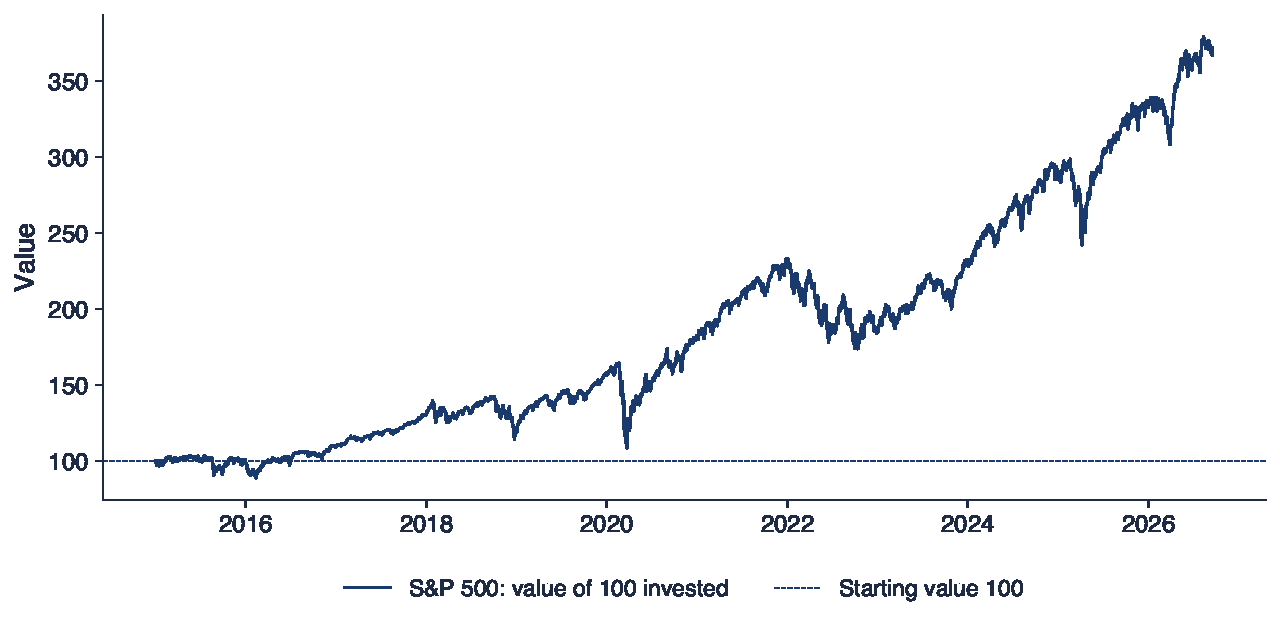
\includegraphics[width=0.94\textwidth,height=0.6\textheight,keepaspectratio]{ch0_sem_b1_growth.pdf}
\end{center}
\vspace{-2mm}
\begin{itemize}
    \item 100 invested on 2 January 2015 were worth 372 on 18 September 2026 (price index, without dividends)
\end{itemize}
\sfmquantlet{Ch_00}{SFM_ch0_seminar}
\end{frame}

\begin{frame}{B1 [Solved]: Solution (3/3) --- Drawdown and Interpretation}
\itemsize{\footnotesize}
\begin{columns}[T]
\begin{column}{0.55\textwidth}
\begin{center}
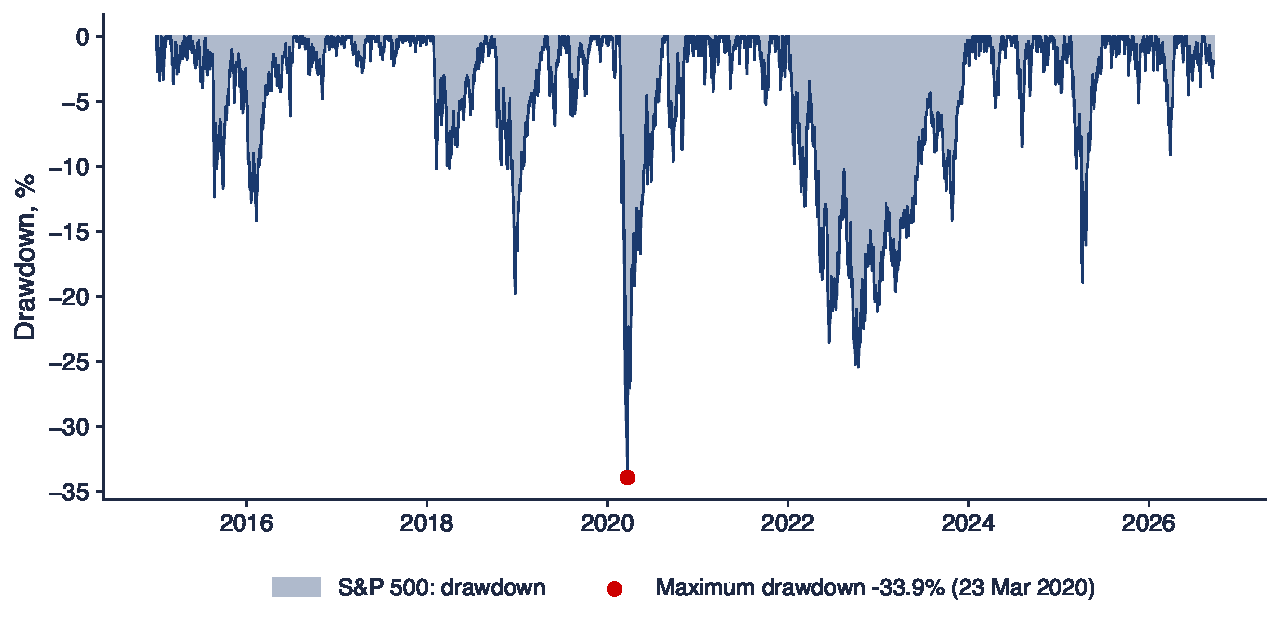
\includegraphics[width=0.94\textwidth,height=0.55\textheight,keepaspectratio]{ch0_sem_b1_drawdown.pdf}
\end{center}
\vspace{-2mm}

\end{column}
\begin{column}{0.42\textwidth}
\begin{itemize}
    \item \textbf{Maximum drawdown}: -33.9\%, from the peak of 19 February 2020 to 23 March 2020 (COVID-19)
    \item Second deepest episode: 2022, when interest rates rose
    \item \textbf{Interpretation}
    \begin{itemize}
        \item a good average year (11.2\%) hides a fall of a third in one month
        \item report the volatility and the drawdown next to the mean
    \end{itemize}
\end{itemize}
\end{column}
\end{columns}
\sfmquantlet{Ch_00}{SFM_ch0_seminar}
\end{frame}

\begin{frame}{B2 [Solved]: One Suspicious Quote --- Task}
\itemsize{\small}
\begin{itemize}
\item \textbf{Question}: is the largest EUR/RON move in the market series a real price?
\item \textbf{Inputs}: the EUR/RON series from EODHD (\texttt{eurron\_eodhd}) and the BNR reference rate (\texttt{eurron}), 2015--2026
\item \textbf{Tasks}
\begin{enumerate}
    \item For each day, compute the gap between the EODHD quote and the BNR rate of the same day, in percent.
    \item Find the day with the largest absolute gap, and print the quotes of the day before and the day after.
    \item Compute the log returns into and out of that day.
    \item Plot both series in the month around that day.
\end{enumerate}
\item \textbf{Report}: the date, the quote, the BNR rate, the two log returns, and your decision: real price or bad tick
\item Notebook: section B2
\end{itemize}
\end{frame}

\begin{frame}{B2 [Solved]: Solution (1/2) --- Step by Step}
\itemsize{\small}
\begin{itemize}
    \item \textbf{Largest gap}: 13 August 2025
    \begin{itemize}
        \item EODHD quote 5.9065 against the BNR rate 5.0633: a gap of +16.7\%
        \item day before (12 August 2025): 5.0636; day after (14 August 2025): 5.0629
    \end{itemize}
    \item \textbf{Two log returns}
    \begin{itemize}
        \item into the day: +15.4\%; out of the day: -15.4\%
        \item for comparison, the largest daily move of the BNR rate since 2015 is 1.4\%
    \end{itemize}
    \item \textbf{Decision}: a bad tick
    \begin{itemize}
        \item a jump of 15\% that fully reverses the next day, absent from the official rate
        \item kept in the data, it would add two of the largest daily moves of the leu in a decade
    \end{itemize}
    \item In the course we use the BNR rate for EUR/RON
\end{itemize}
\sfmquantlet{Ch_00}{SFM_ch0_seminar}
\end{frame}

\begin{frame}{B2 [Solved]: Solution (2/2) --- Chart and Interpretation}
\itemsize{\footnotesize}
\begin{center}
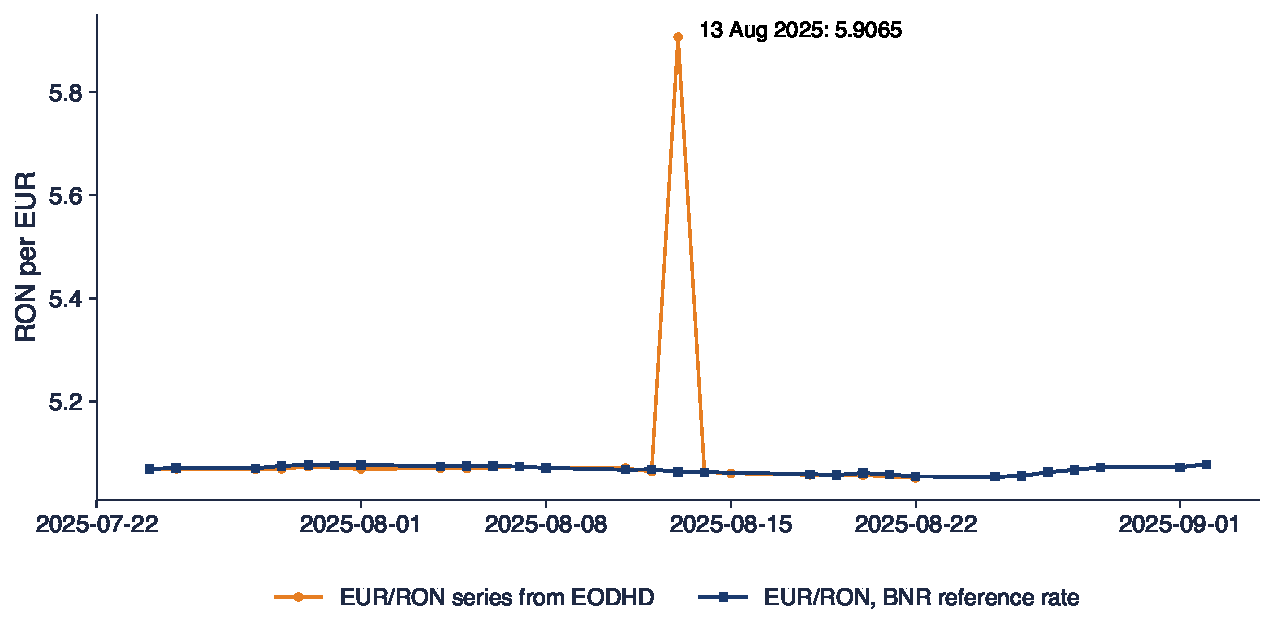
\includegraphics[width=0.94\textwidth,height=0.58\textheight,keepaspectratio]{ch0_sem_b2_eurron.pdf}
\end{center}
\vspace{-2mm}
\begin{itemize}
    \item One quote far from every other quote and from the official rate: always look at the data before computing statistics
    \item Interpretation: a volatility computed with this tick would describe an error, not the market
\end{itemize}
\sfmquantlet{Ch_00}{SFM_ch0_seminar}
\end{frame}


%=============================================================================
\section{Your Turn}
%=============================================================================

\begin{frame}{A4 [Proposed]: New Numbers --- Task}
\itemsize{\small}
\begin{itemize}
\item \textbf{Question}: can you repeat A1--A3 without the solution in front of you?
\item \textbf{Inputs}: a share at $P_0 = 50$, $P_1 = 55$, $P_2 = 44$; a fund at 200, 180, 220, 165, 198, 230 on days 0--5; daily mean $0.03\%$ and daily volatility $1.5\%$
\item \textbf{Tasks}
\begin{enumerate}
    \item Model: A1, A2 and A3 [Solved].
    \item Compute the two simple and the two log returns of the share, their sums and the two-day returns.
    \item Compute the drawdown of the fund for each day and its maximum drawdown.
    \item Annualise the daily mean and volatility with $q = 252$.
\end{enumerate}
\item \textbf{Report}: the two tables, the maximum drawdown, the two annual numbers, and one sentence on which return sum matches the two-day return
\item Notebook: section A4
\end{itemize}
\end{frame}

\ifsolutions
\begin{frame}{A4: Solution (Instructor)}
\itemsize{\small}
\begin{itemize}
    \item \textbf{Share}
    \begin{itemize}
        \item $R_1 = +$10.00\%, $R_2 = $ -20.00\%; $r_1 = +$9.53\%, $r_2 = $ -22.31\%
        \item sums: -10.00\% (simple), -12.78\% (log); two-day: -12.00\% (simple), -12.78\% (log)
        \item only the log sum equals the two-day log return
    \end{itemize}
    \item \textbf{Fund}
    \begin{itemize}
        \item $DD_t$: 0.0, -10.0, 0.0, -25.0, -10.0, 0.0 (\%)
        \item maximum drawdown -25.0\%, from 220 (day 2) to 165 (day 3); a new peak on day 5
    \end{itemize}
    \item \textbf{Annualisation}
    \begin{itemize}
        \item mean $252 \times 0.03\% = $ 7.6\%; volatility $\sqrt{252} \times 1.5\% = $ 23.8\%
    \end{itemize}
\end{itemize}
\end{frame}
\fi

\begin{frame}{B3 [Proposed]: The BET-TR, 2015--2026 --- Task}
\itemsize{\small}
\begin{itemize}
\item \textbf{Question}: how did the Romanian market with dividends compare with the S\&P 500?
\item \textbf{Inputs}: BET-TR closing prices from 2 January 2015 (\texttt{load\_close('bettr')}) to 18 September 2026
\item \textbf{Tasks}
\begin{enumerate}
    \item Model: B1 [Solved]; reuse its code and change only the series name.
    \item Compute $q$, the annualised mean log return and the annualised volatility.
    \item Compute the cumulative return and the maximum drawdown with its dates.
    \item Compare each number with the S\&P 500 result of B1.
\end{enumerate}
\item \textbf{Report}: a two-column table (S\&P 500, BET-TR) and one sentence: why is the comparison not fully fair?
\item Notebook: section B3
\end{itemize}
\end{frame}

\ifsolutions
\begin{frame}{B3: Solution (Instructor)}
\itemsize{\small}
\begin{columns}[T]
\begin{column}{0.45\textwidth}
\begin{center}
\footnotesize
\begin{tabular}{lrr}
\toprule
& S\&P 500 & BET-TR \\
\midrule
$q$ & 251.5 & 250.0 \\
mean, \% a year & 11.2 & 20.0 \\
volatility, \% a year & 17.7 & 15.5 \\
cumulative, \% & 271.7 & 938.5 \\
MDD, \% & -33.9 & -31.1 \\
\bottomrule
\end{tabular}
\end{center}

\end{column}
\begin{column}{0.52\textwidth}
\begin{itemize}
    \item BET-TR: maximum drawdown from 23 January 2020 to 23 March 2020
    \item \textbf{Interpretation}
    \begin{itemize}
        \item BET-TR: higher mean, lower volatility in this window
        \item not fully fair: BET-TR includes dividends, the S\&P 500 price index does not; currencies differ (RON, USD)
    \end{itemize}
\end{itemize}
\end{column}
\end{columns}
\end{frame}
\fi

\begin{frame}{B4 [Proposed]: Bitcoin: 365 or 252 Days? --- Task}
\itemsize{\small}
\begin{itemize}
\item \textbf{Question}: how large is the error if Bitcoin is annualised like a stock index?
\item \textbf{Inputs}: Bitcoin closing prices from 2 January 2015 (\texttt{load\_close('btc')}) to 18 September 2026
\item \textbf{Tasks}
\begin{enumerate}
    \item Model: A2 and B1 [Solved].
    \item Compute the number of returns per year $q$ from the data.
    \item Compute the annualised volatility with $q = 365$, and then with $q = 252$.
    \item Compute the cumulative return and the maximum drawdown with its dates.
\end{enumerate}
\item \textbf{Report}: $q$, the two volatilities and their ratio, the cumulative return, the maximum drawdown, and one sentence on which volatility is right
\item Notebook: section B4
\end{itemize}
\end{frame}

\ifsolutions
\begin{frame}{B4: Solution (Instructor)}
\itemsize{\small}
\begin{itemize}
    \item 4\,277 daily returns: $q = $ 365.3, so 365 is right
    \item \textbf{Volatility}
    \begin{itemize}
        \item with 365: 66.7\% a year; with 252: 55.4\% a year
        \item ratio $\sqrt{365/252} = $ 1.20: using 252 understates the risk by about a sixth
    \end{itemize}
    \item \textbf{Return and drawdown}
    \begin{itemize}
        \item annual mean 47.4\%; cumulative return 25580.4\% (price $\times$257)
        \item maximum drawdown -83.4\%, from 16 December 2017 to 15 December 2018
    \end{itemize}
    \item Interpretation: huge growth and a loss of 83\% within one year are both part of the same series
\end{itemize}
\end{frame}
\fi


%=============================================================================
\section{Part C: Critique an AI Answer}
%=============================================================================

\begin{frame}[fragile]{C2 [Proposed]: Critique an AI Answer --- the Answer}
\itemsize{\footnotesize}
\begin{itemize}
    \item \textbf{Prompt} sent to an AI assistant: ``From the course data, compute the annualised volatility and the cumulative return of the S\&P 500 and of Bitcoin since 2 January 2015, from daily simple returns.''
\end{itemize}
\begin{lstlisting}
# read_market(symbol): the daily table of the course data
for name, sym in [('S&P 500', 'GSPC.INDX'), ('Bitcoin', 'BTC-USD.CC')]:
    p = read_market(sym)['close'].loc['2015-01-02':]   # closing prices
    R = p.pct_change().dropna()          # daily simple returns
    vol = R.std() * 252                  # annualised volatility
    cum = R.sum()                        # cumulative return
    print(name, round(100 * vol, 1), round(100 * cum, 1))
\end{lstlisting}
\begin{itemize}
    \item \textbf{Conclusion of the AI}: ``Volatility: S\&P 500 280.3\%, Bitcoin 873.3\%. Cumulative return: S\&P 500 149.6\%, Bitcoin 814.0\%. Bitcoin earned only about five times as much as the S\&P 500.''
\end{itemize}
\end{frame}

\begin{frame}{C2 [Proposed]: Critique an AI Answer --- Task}
\itemsize{\small}
\begin{itemize}
\item \textbf{Question}: can you trust code that runs without an error message?
\item \textbf{Inputs}: the code and the conclusion on the previous slide; the definitions of the primer
\item \textbf{Tasks}
\begin{enumerate}
    \item Model: A1, A2 and B1 [Solved].
    \item Find the three errors planted in the code.
    \item For each error, say how you would detect it: a check on the output, the primer, or a solved exercise.
    \item Write the corrected code, and report the corrected volatility and cumulative return of both assets.
    \item Say whether the conclusion ``Bitcoin earned only about five times as much'' survives.
\end{enumerate}
\item \textbf{Report}: a table AI versus corrected, and one line per error in the format: request, answer, error, how found, correction
\item Notebook: section C2
\end{itemize}
\end{frame}

\ifsolutions
\begin{frame}{C2: Solution (Instructor)}
\itemsize{\footnotesize}
\begin{columns}[T]
\begin{column}{0.50\textwidth}
\begin{itemize}
    \item \textbf{Error 1}: \texttt{R.std() * 252}; volatility scales with $\sqrt{252}$
    \begin{itemize}
        \item detect: a volatility of 280.3\% a year for a stock index is impossible (A2)
    \end{itemize}
    \item \textbf{Error 2}: 252 days for Bitcoin, which trades every day
    \begin{itemize}
        \item detect: count the observations per year (365.3)
    \end{itemize}
    \item \textbf{Error 3}: \texttt{R.sum()} is not the cumulative return; simple returns compound
    \begin{itemize}
        \item detect: compare with $P_T/P_0 - 1$ (A1, B1)
    \end{itemize}
\end{itemize}
\end{column}
\begin{column}{0.47\textwidth}
\begin{center}
\footnotesize
\begin{tabular}{lrr}
\toprule
& Vol. \% & Cum. \% \\
\midrule
S\&P 500, AI & 280.3 & 149.6 \\
S\&P 500, corrected & 17.7 & 271.7 \\
Bitcoin, AI & 873.3 & 814.0 \\
Bitcoin, corrected & 66.2 & 25580.4 \\
\bottomrule
\end{tabular}
\end{center}
\begin{itemize}
    \item Corrected: \texttt{R.std() * np.sqrt(q)} with $q$ = 252 or 365, and \texttt{p.iloc[-1] / p.iloc[0] - 1}
    \item The conclusion fails: Bitcoin earned about 94.1 times as much as the S\&P 500, not 5.4 times, with 3.7 times the volatility
\end{itemize}
\end{column}
\end{columns}
\end{frame}
\fi


%=============================================================================
\section{Wrap-up}
%=============================================================================

\begin{frame}{Practice at Home}
\itemsize{\small}
\begin{itemize}
    \item \textbf{Finish the proposed exercises}: A4, B3, B4 and C2
    \begin{itemize}
        \item each names its model, a solved exercise to copy
        \item the solutions are discussed at the next seminar
    \end{itemize}
    \item \textbf{Try one more series}
    \begin{itemize}
        \item repeat B1 for the DAX (\texttt{dax}) or for gold (\texttt{gold}), and compare the annual volatilities
    \end{itemize}
    \item \textbf{Take the \sfmchlink{https://danpele.github.io/SFM/EN/Courses/chapter0_introduction.pdf}{Chapter 0} quiz} on the course website: 20 questions, each answer explained
    \item Nothing is handed in: this is practice for the exam and for the project
\end{itemize}
\end{frame}

\begin{frame}{Recap, and Next: the \sfmchlinkt{https://danpele.github.io/SFM/EN/Courses/chapter0_introduction.pdf}{Chapter 0} Lecture}
\itemsize{\small}
\begin{columns}[T]
\begin{column}{0.52\textwidth}
\begin{itemize}
    \item \textbf{Today}
    \begin{itemize}
        \item simple returns compound, log returns add up
        \item annualise the mean with $q$ and the volatility with $\sqrt{q}$; $q = 365$ for Bitcoin
        \item the maximum drawdown is the worst loss from a peak
        \item look at the data first: one bad tick can dominate a statistic
        \item AI code can run and still be wrong
    \end{itemize}
\end{itemize}
\end{column}
\begin{column}{0.45\textwidth}
\begin{itemize}
    \item \textbf{In the lecture}
    \begin{itemize}
        \item How is the course organised and graded?
        \item What do the 2026 markets look like in the data?
        \item How did exchanges, crashes and models develop?
        \item Why are daily returns not Normal?
    \end{itemize}
\end{itemize}
\end{column}
\end{columns}
\end{frame}

\end{document}
